\chapter{Differential Geometry}
\chapterauthor{Ivo Iliev\\Sofia University}
\adjustmtc
\minitoc
\section{General}
\begin{definition}[Einstein Manifold]
A Riemannian manifold $M$ is called an \textit{Einstein manifold} if its Ricci tensor is proportional to the metric, i.e.
\begin{equation}
Ric_g = \lambda g
\end{equation}
\end{definition}
\begin{remark}
An Einsteinian manifold, where $\lambda=0$ is called a \textit{Ricci-flat} manifold.
\end{remark}

\section{Differential Forms}
\epigraph{"Hamiltonian mechanics cannot be understood without differential
forms"}{V. I. Arnold}

In this section we will give a very brief introduction to differential forms
and the general rules for calculus with differential forms. 
\subsection{Exterior forms}
We begin with the more general notion of a \textit{exterior form}, which is
generally a poly-linear map from a vector space to an algebraic filed.
\subsubsection{Definitions}
Let $\mathbb{L}^n$ be an $n$-dimensional real vector space.
\begin{definition}[Exterior algebraic form of degree $k$]
An exterior algebraic form of degree $k$, also known as a $k$-form, is
a function of $k$ vectors which is $k$-linear and anti-symmetric. Namely:
\begin{equation}
  \omega(\lambda_1\xi_1' + \lambda_2\xi_1'',\xi_2,\cdots,\xi_k)
  = \lambda_1\omega(\xi_1',\xi_2,\cdots,\xi_k)
  + \lambda_2\omega(\xi_1'',\xi_2,\cdots,\xi_k),
\end{equation}
and
\begin{equation}
  \omega(\xi_{i_1},\cdots,\xi_{i_k}) = (-1)^\nu\omega(\xi_1,\cdots,\xi_k)
\end{equation}
with $(-1)^\nu = 1$ if the permutation $(i_1,\cdots,i_k)$ is even and  $(-1)^\nu
= -1$ if the same permutation is odd. Here, $\xi_i\in\mathbb{L}^n$ and
$\lambda_i\in\mathbb{R}$.
\end{definition}
The set of all $k$-forms in $\mathbb{L}^n$ forms a real vector space. Indeed,
one has that:
\begin{equation}
   (\omega_1+\omega_2)(\xi) = \omega_1(\xi) + \omega_2(\xi), \quad \xi
   = \{\xi_1,\cdots,\xi_k\}
\end{equation}
and
\begin{equation}
  (\lambda\omega)(\xi) = \lambda\omega(\xi).
\end{equation}
Since $\mathbb{L}^n$ is a vector space, we can always suppose that it is
equipped with a coordinate system. Let us denote these coordinates by
$x_1,\cdots,x_n$. Now, we can think of these coordinates as 1-forms so that
$x_i(\xi) = \xi_i$ and that is the $i$-th coordinate of the vector $\xi$. These
coordinates form a basis of 1-forms in the 1-form vector space (which is also
called the \textit{dual space} $(\mathbb{L}^n)^*$).
\par Any 1-form can then be
written as a linear combination of basis 1-forms:
\begin{equation}
  \omega_1 = a_1x_1 + \cdots + a_nx_n.
\end{equation}

\subsubsection{Exterior Products}
\begin{definition}[Exterior Product]
An exterior product of $k$ 1-forms $\omega_1,\omega_2,\cdots,\omega_k$ is
a $k$-form defined by
\begin{equation}
  (\omega_1\wedge\omega_2\wedge\cdots\wedge\omega_k)(\xi_1,\xi_2,\cdots,\xi_k)
  = det\omega_i(\xi_j).
\end{equation}
\end{definition}
\begin{remark}
  Exterior products of basis 1-forms $x_{i_1}\wedge\cdots\wedge x_{i_k}$ with
  $i_1<\cdots<i_k$ for a basis in the space of $k$-forms. The dimension the latter
  space is obviously $C_n^k$.
\end{remark}
A general $k$-form can be written as
\begin{equation}
  \omega^k = \sum_{1\leq i_1<\cdots<i_k\leq n}{a_{i_1\cdots
  i_k}x_{i_1}\wedge\cdots\wedge x_{i_k}}
\end{equation}
where $a_{i_1\cdots i_k}$ are real numbers.

\begin{definition}[Exterior product of an $k$-form and an $l$-form]
  The exterior product $\omega^k\wedge\omega^l$ of a $k$-form with an $l$-form
  on $\mathbb{L}^n$ is the $k+l$-form on $\mathbb{L}^n$ defined as:
  \begin{equation}
    (\omega^k\wedge\omega^l)(\xi_1,\cdots,\xi_{k+l})
    = \sum{(-1)^\nu\omega^k(\xi_{i_1},\cdots,\xi_{i_k})\wedge\omega^l(\xi_{j_1},\cdots,\xi_{j_l})}
  \end{equation}
  where $i_1<\cdots<i_k$ and $j_1,<\cdots<j_l$ and the sum is taken over all
  permutations $(i_1,\cdots,i_k,j_1,\cdots,j_l)$ with $(-1)^\nu$ being +1
  for even permutations and -1 for odd permutation.
\end{definition}
One can check that this definition is consistent with the definition for
exterior product of 1-forms. Furthermore it can be shown that the exterior
product is distributive, associative and \textit{skew-commutative}. The latter
means that $\omega^k\wedge\omega^l = (-1)^{kl}\omega^l\wedge\omega^k$. If
$\omega$ is a 1-form (or a form of any odd degree) one can easily show that
$\omega\wedge\omega=0$. We will present a brief version of the proof here:
\begin{proof}
Let $\omega$ be an exterior $k$-form, where $k$ is an odd integer. Then the
exterior product takes the form:
 \begin{equation}
 \omega\wedge\omega = (-1)^{k^2}\omega\wedge\omega
 \end{equation}
 But $k$ is odd, therefore $k^2$ is odd. From that we see that
 \begin{equation}
   \omega\wedge\omega = (-1)^{k^2}\omega\wedge\omega = -\omega\wedge\omega
 \end{equation}
 From this we conclude that $\omega\wedge\omega = 0$.
\end{proof}
\subsubsection{Behaviour under mappings}
Let $f:\mathbb{L}^m\rightarrow\mathbb{L}^n$ be a linear map and $\omega^k$ an
exterior $k$-form on $\mathbb{L}^n$. We can define a $k$-form $(f^*\omega^k)$
on $\mathbb{L}^m$ by
\begin{equation}
  (f^*\omega^k)(\xi_1,\cdots,\xi_k) = \omega^k(f\xi_1,\cdots,f\xi_k)
\end{equation}
Notice that the obtained mapping of forms $f^*$ acts in \textit{opposite}
direction to $f$. Namely,
$f^*:\Omega_k(\mathbb{L}^n)\rightarrow\Omega_k(\mathbb{L}^b)$, where
$\Omega_k(\mathbb{L}^n)$ is the vector space of $k$-forms on $\mathbb{L}^n$.
\subsection{Differential Forms}
After the general discussion about exterior forms it is time to restrict
ourselves to a more practical object, namely the differential form.
Understanding differential forms or at least having working knowledge about the
topic is paramount for the study of differential geometry and physics on curved
manifolds. Although this may seem abstract at first, we urge the reader to push
through the mathematical definitions and grasp the essence of the idea, that is
how do we perform calculus on curved manifolds without the notion of
coordinates. 
\begin{definition}[Differential Form]
  A differential $k$-form $\omega^k\vert_x$ at a point $x$ of a manifold $M$ is
  an exterior $k$-form on the tangent space $TM_x$ to $M$ at $x$, i.e.,
  a $k$-linear skew-symmetric function of $k$ vectors $\xi_1,\cdots,\xi_k$
  tangent to $M$ at $x$. If such a form is given at every point $x$ of $M$ and
  if it is differentiable, we say that we are given a $k$-form $\omega^k$ on
  the manifold $M$.
\end{definition}
We intoduce the coordinate basis 1-forms $dx_i$ with $i=1,\cdots,n$ $(dimM
= n)$. The notation $dx_i$ is used for the exterior forms emphasizes that these
basis forms act on $TM_x$ at a given point $x$ of $M$. In the neighborhood of
$x$ one can always write the general differential $k$-form as
\begin{equation}
  \omega^k
  = \sum_{i_1<\cdots<i_k}{a_{i_1,\cdots,i_k}(x)dx_{i_1}\wedge\cdots\wedge
  dx_{i_k}},
  \label{eq:generaldifferentialform}
\end{equation}
where $a_{i_1\cdots i_k}$ are smooth functions of $x$. Let's give a simple
example.
\begin{example}
  The differential of some scalar function $f(x)$ defined on a manifold $M$ is
  a differential 1-form. We introduce
  \begin{equation}
    df = \sum_{k=1}^n{\frac{\partial f}{\partial x_k}\bigg\vert_x dx_k},
  \end{equation}
where $dx_k$ are basis differential 1-forms. The value of this 1-form on
a vector $\xi\in TM_x$ is given by
\begin{equation}
  df(\xi) = \sum_{k=1}^n{\frac{\partial f}{\partial x_k}\bigg\vert_x \xi_k}.
\end{equation}
\end{example}
\subsubsection{Behaviour under mappings}
Let $f:M\rightarrow N$ be a differentiable map of a smooth manifold $M$ to
a smooth manifold $N$, and let $\omega$ be a differential $k$-form o $N$. The
mapping $f$ induces the mapping $f_*:TM_x\rightarrow TM_{f(x)}$ of tangent
spaces. The latter mapping $f_*$ is called the \textit{differential} of the map
$f$. The mapping $f_*$ is a mapping of linear spaces and gives rise to the
mapping of forms defined on corresponding tangent spaces. As a result
a well-defined differential $k$-form $(f^*\omega)$ exists on $M$:
\begin{equation}
  (f^*\omega)(\xi_1,\cdots,\xi_k) = \omega(f_*\xi_1,\cdots,f_*\xi_k).
\end{equation}
\subsection{Integration of Differential Forms over Chains}
\subsubsection{Integration of $k$-form over $k$-dimensional cell}
Let $D$ be a bounded convex polyhedron in $\mathbb{L}^k$ and $x_1,\cdots,x_k$
an oriented coordinate system on $\mathbb{L}^k$. Any differential $k$-form on
$\mathbb{L}^k$ can be written as $\omega^k=\phi(x)dx_1\wedge\cdots\wedge dx_k$,
where $\phi(x)$ is a differentiable function on $\mathbb{R}^k$. We define
the integral of the form $\omega^k$ over $D$ as the integral of the function
$\phi(x)$:
\begin{equation}
  \int_D{\omega_k} = \int_D{\phi(x)dx_1dx_2\cdots dx_k}.
\end{equation}

\begin{definition}[$k$-dimensional cell]
A $k$-dimensional cell $\sigma$ of an $n$-dimensional manifold $M$ is
a polyhedron $D$ in $\mathbb{L}^n$ with a differentiable map $f:D\rightarrow
M$.
\end{definition}
One can think about $\sigma$ as a "curvilinear polyhedron" - the image of $D$
on $M$. If $\omega$ is a differentiable $k$-form on $M$, we define the integral
of a form over the cell $\sigma$ as
\begin{equation}
  \int_\sigma{\omega} = \int_D{f^*\omega},
\end{equation}
where $f^*$ is a mapping of $k$-forms induced by $f$.
\par The cell $\sigma$ inherits an orientation from the orientation of
$\mathbb{L}^k$. The $k$-dimensional cell which differs from $\sigma$ only by
the choice of orientation is called the \textit{negative} of $\sigma$ and is
denoted by $-\sigma$ or by $(-1)\sigma$. One can show that under a change of
orientation the integral changes sign:
\begin{equation}
  \int_{-\sigma}{\omega}=-\int_{\sigma}{\omega}.
\end{equation}

\subsubsection{Chains and the Boundary Operator}
It is convenient to generalize our definition of the integral of a form over
\textit{cell} to the integral over a \textit{chain}.
\begin{definition}[Chain of a Manifold]
  A chain of dimension $k$ on a manifold $M$ consists of a finite collection of
  $k$-dimensional oriented cells $\sigma_1,\cdots,\sigma_r$ in $M$ and integers
  $m_1,\cdots,m_r$ called multiplicities. A chains is denoted by
  \begin{equation}
    c_k = m_1\sigma_1+\cdots+m_r\sigma_r .
  \end{equation}
\end{definition}
One can introduce the structure of a commutative group on a set of $k$-chains
on $M$ with natural definitions of addition of chains $c_k + b_k$.
\begin{definition}[Boundary Operator]
  The boundary of a convex oriented $k$-polyhedron $D$ on $\mathbb{L}^k$ is the
  $(k-1)$-chain $\partial D$ on $\mathbb{L}^k$ defined as
  \begin{equation}
    \partial D = \sum_i{\sigma_i}
  \end{equation}
  where the cells $\sigma_i$ are the $(k-1)$-dimensional faces of $D$ with
  orientations inherited from the orientation of $\mathbb{L}^k$.
\end{definition}

One can easily extend this definition to the definition of the \textit{boundary
of a cell} $\partial\sigma$ on $M$ and then to the boundary of a chain. Indeed,
defining:
\begin{definition}[Boudary of a Chain]
  \begin{equation}
    \partial c_k = m_1\partial\sigma_1 + \cdots + m_r\partial\sigma_r
  \end{equation}
\end{definition}
We can see that $\partial c_k$ is a $(k-1)$-chain on $M$. Additionally, we
define a 0-chain as a collection of points with multiplicities. Furthermore we
define the boundary of an oriented interval $\vec{AB}$ as $B-A$. The boundary
of a point is empty.
\par It is straightforward to show that the boundary of the boundary of a cell
is zero. Therefore 
\begin{equation}
  \partial(\partial c_k) = 0
\end{equation}
for any $k$-chain $c_k$. We denote this property as
\begin{equation}
  \partial\partial = \partial^2 = 0
\end{equation}
\subsubsection{Integration of a $k$-form over a $k$-chain}
An integral of a $k$-form over a $k$-chain is then defined as
\begin{equation}
  \int_{c_k}{\omega^k} = \sum{m_i\int_{\sigma_i}{\omega^k}}.
\end{equation}
\subsection{Exterior Differentiation and Stokes Formula}
\begin{definition}[Exterior Derivative of a Form]
  An \textit{exterior derivative} of a differential $k$-form $\omega$ is
  a $(k+1)$-form $\Omega=d\omega^k$. Given a set of coordinates $\{dx_{i_j}\}$,
  we have:
  \begin{equation}
    \Omega = d\omega^k = \sum{da_{i_1\cdots i_k}\wedge
      dx_{i_1}\wedge\cdots\wedge dx_{i_k}}
    \end{equation}
    implying that we have defined $\omega^k$ as in
    \eqref{eq:generaldifferentialform}. Here, $da$ is a 1-form, the
    differential of the function $a(x)$.
\end{definition}
One can show that the definition does not actually depend on the choice of
coordinates. We can think of the 1-form given by the differential of a scalar
function as of an external derivative of a 0-form.
It is easy to show that $d(df)=0$, if $f$ belongs to the set of 0-forms. Indeed
\begin{proof}
  If f belongs to the set of 0-forms, then by definition
  \begin{equation}
   df = \sum{\frac{\partial a}{\partial x^i}dx^i},
  \end{equation}
  which is a 1-form. Taking an exterior derivative again yields
  \begin{align}
     d(df) &= d\left(\sum{\frac{\partial a}{\partial x^i}dx^i}\right)=\nonumber\\
    &= \sum{\frac{\partial^2}{\partial x^i\partial x^j}dx^i\wedge x^j}
     =\nonumber\\
    &= \frac{\partial^2 g}{dx^i dx^j}dx^i\wedge dx^j + \frac{\partial^2 g}{dx^j
    dx^i}dx^j\wedge dx^i\nonumber\\
    &= 0
  \end{align}
  Here we have used that $\frac{\partial g^2}{dx^i dx^j} = \frac{\partial
  g^2}{dx^j dx^i}$ and $dx^i\wedge dx^j = -dx^j\wedge dx^i$.
\end{proof}
Using this result, one can show that it holds for forms of any degree.
\par Another useful formula is that for differentiating an exterior product of
form:
\begin{equation}
  d(\omega^k\wedge\omega^l) = d\omega^k\wedge d\omega^l + (-1)^k\omega^k\wedge
  d\omega^l
\end{equation}
\par Lastly, if $f:M\rightarrow N$ is a smooth map and $\omega$ is a $k$-form
on $N$, we have
\begin{equation}
  f^*(d\omega) = d(f^*\omega).
\end{equation}
\subsubsection{Stokes' Formula}
One of the most-important formulae in differential geometry is the
\textit{Newton-Leibniz-Gauss-Green-Ostrogradski-Stokes-Poincar\'e} formula:
\begin{equation}
  \boxed{\int_{\partial c}{\omega} = \int_c{d\omega}}
\end{equation}
where $c$ is any $(k+1)$-chain on a manifold $M$ and $\omega$ is any $k$-form
on M. In the case when the boundary $\partial c=0$, we have $\int_c{d\omega}
= 0$, which corresponds to integration of a complete derivative over a closed
surface.
\subsection{Homologies and Cohomologies}
\subsubsection{Closed and Exact Forms}
\begin{definition}[Closed Form]
  A differential form $\omega$ on a manifold $M$ is said to be \textit{closed}
  if $d\omega = 0.$
\end{definition}
In particular, on a 3D Riemannian manifold, we have $d\omega^2_{\vec{A}}
= \left(\nabla\cdot\vec{A}\right)\omega^3 = 0$, which is equivalent to
$\left(\nabla\cdot\vec{A}\right) = 0$, i.e the corresponding vector field is
divergenless. We can apply Stokes' formula for a closed form, getting
\begin{equation}
  \int_{\partial c_{k+1}}{\omega^k} = 0\quad\text{if }dw^k=0.
  \label{eq:stokesclosedform}
\end{equation}
\begin{definition}[Exact Form]
  A  differential form $\omega$ on a manifold $M$ is said to be \textit{exact}
  if there exists such a differential form $\mu$ that $\omega = d\mu$.
\end{definition}
Since $d(d\omega) = 0$ as we've proven all exact forms are closed. However,
there are some closed forms which are not exact. Let's give a short example.
\begin{example}
  Consider the circle $S^1$, parametrized by an angle $\phi\in [0,2\pi]$. One
  can introduce the 1-form $\omega^1$, defined by
  $\omega^1(\partial_t\gamma)=\partial_t\gamma$, where $\partial_t\gamma$ is
  the "velocity" along the path $\phi = \gamma(t)$. Obviously, this "velocity",
  belongs to the tangent space of $S^1$ at the point with coordinate $\phi$.
  The form is closed - $d\omega$ is a 2-form, and we can't have 2-forms on
  a one-dimensional manifold. However:
  \begin{equation}
    \int_{S^1}\omega^1 = \int_{0}^T{dt \partial_t\gamma} = 2\pi,
  \end{equation}
the length of the circle. Although the boundary $\partial S^1$ is zero, the
integral is not zero, and therefore $\omega^1$ is not exact.
\end{example}
\par One can notice that locally the introduced 1-form can be written as
$\omega^1 = d\phi$, which can look like a contradiction. It is easy to see
where the problem lies - writing $\omega^1 = d\phi$ is not valid for $\phi=0$.
We've come across an example of a general result, namely
\begin{theorem}[Poincar\'e's Lemma]
  Any closed form is locally exact.
\end{theorem}
The existence of locally but not globally exact closed forms is related to some
topological properties of the underlying manifold $M$.

\begin{subsubsection}{Cycles and Boundaries}
  \begin{definition}[Cycle on a Manifold]
    A \textit{cycle} on a manifold $M$ is a chain whose boundary is equal to
    zero.
  \end{definition}
  Using Stokes theorem, we have
  \begin{equation}
    \int_{c_{k+1}}{d\omega^k} =0\quad \text{if } \partial c_{k+1} =0.
  \end{equation}
  Chains that can be considered boundaries of some other chains are called
  \textit{boundaries}. Since $\partial\partial = 0$, all boundaries are cycles.
  However, not all cycles are boundaries. The existence of cycles that are not
  boundaries is again related to some topological properties of the manifold.
  A fairly simple example is found on the 2-torus. The 2-torus is the direct
  product of 2 circles - $T^2=S^1\cross S^1$. Each of the $S^1$ is a cycle, but
  none of them are boundaries. 

  \begin{subsubsection}{Homologies and Cohomologies}
  The set of all $k$-forms on $M$ is a vector space, the set of all
  \textit{closed} $k$-forms is a subspace of that space and the set of
  differentials of $(k-1)$-forms (the \text{exact} $k$-forms) are a subspace of
  the subspace of closed forms. We can now define:
  \begin{definition}
    The quotient space:
  \begin{equation}
    \frac{(\text{closed forms})}{(\text{exact forms})} = H^k(M,\mathbb{R})
  \end{equation}
    is called the \textit{k-th cohomology group} of the manifold $M$. An
    element of this group is a class of closed forms, differing from each other
    only by an exact form.
  \end{definition}
  For the circle $S^1$, we have $H^1(S^1,\mathbb{R}) = \mathbb{R}$.
  \begin{definition}[Betti Number]
    The dimension of $H^k$ is called the $k$-th \textit{Betti number} of $M$.
  \end{definition}
  Obviously, the first Betti number of $S^1$ is 1. The cohomology groups of $M$ are important \textit{topological}
  properties of $M$.

  \begin{definition}[Homologous Cycles]
  Let us now consider two $k$-cyclces $a$ and $b$, such that their 
  difference is a boundary of a $(k+1)$-chain, i.e. $a-b = \partial c_{k+1}$.
  Such cycles are called \textit{homologous}.
\end{definition}
  Let us have two $k$-cycles, $a$ and $b$, homologous to each other and
  a closed form $\omega^k$. From \eqref{eq:stokesclosedform} we can see that 
  \begin{equation}
    \int_a{\omega^k} = \int_b{\omega^k}.
  \end{equation}
  In other words, homologous cycles can be replaced with one another for
  integration paths.
  \begin{definition}[Homology Group]
    The quotient group
    \begin{equation}
      \frac{(\text{cycles})}{(\text{boundaries})} = H_k(M)
    \end{equation}
    is called the $k$-th homology group of $M$. An element of this group is
    a class of cycles homologous to each other. The rank of this group is also
    equal to the $k$-th Betti number of $M$.
  \end{definition}
\subsection{Homologies and Homotopies}
There are important relations between homology and homotopy groups of
a topological space $M$.
\par Let us suppose that $\pi_1(M)$ and $H_1(M)$ are the fundamental and the
first homology group of $M$, respectively. Then $H_1(M)
= \pi_1(M)/[\pi_1,\pi_1]$, where $[\pi_1,\pi_1]$ is the commutator in the
fundamental group. In particular, if $\pi_1(M)$ is Abelian, then $\pi_1(M)
= H_1(M)$. For the higher homotopy groups, there is another result, known as
the Gurevich theorem.
\begin{theorem}[Gurevich theorem]
  If $\pi_k(M) = 0$ for all $k<n$, then
  \begin{equation}
    \pi_n(M) = H_n(M).
  \end{equation}
\end{theorem}
As a general rule of thumb, homology (and cohomology) groups are usually easier
to calculate than homotopy groups.
    \section{Contact Manifolds}
\begin{definition}[Riemannian Cone]
Given a Riemannian manifold $(M,g)$, its \textit{Riemannian cone} is a product
\begin{equation}
(M\times\mathbb{R}^{>0})
\end{equation}
of $M$ with the half-line $\mathbb{R}^{>0}$ equipped with the \textit{cone metric}
\begin{equation}
t^2g+dt^2,
\end{equation}
where t is a parameter in $\mathbb{R}^{>0}$
\end{definition}

\begin{definition}[Contact Manifold]
A manifold $M$, equipped with a 1-form $\theta$ is contact if and only if the 2-form
\begin{equation}
t^2d\theta + 2tdt\cdot\theta
\end{equation}
on its cone is symplectic.
\end{definition}

\begin{definition}[Sasakian Manifold]
A contact Riemannian manifold is called a Sasakian manifold, if its Riemannian cone with the cone metric is a K\"ahler manifold with K\"ahler form
\begin{equation}
t^2d\theta + 2t dt\cdot \theta .
\end{equation}
\end{definition}

\begin{example}
Consider the manifold $\mathbb{R}^{2n+1}$ with coordinates $(\vec{x},\vec{y},z)$, endowed with contact form 
\begin{equation}
\theta = \frac{1}{2}dz + \Sigma_i{y_idx_i}
\end{equation}
and Riemannian metric

\begin{equation}
g = \Sigma_i{(dx_i)^2 + (dy_i)^2 + \theta^2}
\end{equation}
\end{example}

\begin{definition}[Sasaki-Einstein Manifold]
A Sasaki-Einstein manifold is a Riemanian manifold $(S,g)$ that is both Sasakian and Einstein
\end{definition}

\begin{example}
The odd dimensional sphere $S^{2n-1}$, equipped with its standard Einstein metric is a Sasaki-Einstein manifold. In this case, the K\"ahler cone is $\mathbb{C}^2\backslash\{0\}$, equipped with its flat metric.
\end{example}

\section{Symplectic Geometry}
\begin{theorem}[Duistermaat-Heckman Formula]
For a compact symplectic manifold $M$ of dimension $2n$ with symplectic form $\omega$ and with a Hamiltonian $U(1)$ action whose moment map is denoted by $\mu$, the following formula holds:
\begin{equation}
\int_M{\frac{\omega^n}{n!}e^{-\mu}} = \sum_i{\frac{e^{-\mu(x_i)}}{e(x_i)}}
\end{equation}
Here, $x_i$ are the fixed points of the $U(1)$ action and they are assumed to be isolated, and $e(x_i)$ is the product of the weights of the $U(1)$ action on the tangent space at $x_i$.

\end{theorem}

\section{Complex Manifolds}
\begin{definition}[Hermitian Metric]
If a Riemannian metric $g$ of a complex manifold $M$ satisfies 
\begin{equation}
g_p(J_pX, J_pY) = g_p(X,Y)
\end{equation}
at each point $p\in M$ and for any $X,Y\in T_p M$, $g$ is said to be a \textit{Hermitian metric}. Here, $J_p$ denotes the almost complex structure on $M$.
\end{definition}

\begin{definition}[Hermitian Manifold]
The pair $(M,g)$ is called a \textit{Hermitian manifold}
\end{definition}

\begin{theorem}
A complex manifold always admits a Hermitian metric.
\end{theorem}

\begin{proof}
Let $g$ be any Riemannian metric of a complex manifold $M$. Define a new metric $\hat{g}$ by
\begin{equation}
\hat{g}_p(X,Y)\equiv \frac{1}{2}\left[g_p(X,Y) + g_p(J_pX, J_pY)\right].
\end{equation}
Clearly $\hat{g}_p(J_pX,J_pY) = \hat{g}_p(X,Y)$. Moreover, $\hat{g}$ is positive definite provided that $g$ is. Hence, $\hat{g}$ is a Hermitian metric on M
\end{proof}

\begin{definition}[K\"ahler Form]
  Let $(M,g)$ be a Hermitian manifold. Define a tensor field $\Omega$ whose
  action on $X,Y\in T_pM$ is
\begin{equation}
\Omega_p(X,Y) = g_p(J_pX,Y)
\end{equation}
Note that $\Omega$ is anti-symmetric, $\Omega(X,Y) = g(JX,Y) = g(J^2X,JY)
= -g(JY,X) = -\Omega(Y,X)$. Hence, $\Omega$ defines a two-form, called the
\textit{Kh\"aler form} of a Hermitian metric g.
\end{definition}

\begin{definition}[K\"ahler Manifold]
  A \textit{K\"ahler manifold} is a Hermitian manifold $(M,g)$ whose K\"ahler
  form $\Omega$ is closed, $d\Omega=0$. The metric $g$ is called the
  \textit{K\"ahler metric} of M.
\end{definition}

\begin{remark}
Not all complex manifolds admit K\"ahler metrics
\end{remark}

\begin{theorem}
A Hermitian manifold $(M,g)$ is a K\"ahler manifold if and only if the almost
  complex structure $J$ satisfies
\begin{equation}
\nabla_\mu J = 0
\end{equation}
where $\nabla_\mu$ is the Levi-Cevita connection associated with $g$.
\end{theorem}

\begin{proof}
We first note that for any $r$-form $\omega$, d$\omega$ is written as
\begin{equation}
  d\omega = \nabla\omega \equiv
  \frac{1}{r!}\nabla_\mu\omega_{\nu_1\cdots\nu_r}dx^\mu\wedge
  dx^{\nu_1}\wedge\cdots\wedge dx^{\nu}    
\end{equation}
Now we prove that $\nabla_\mu J = 0$ if and only if $\nabla_\mu\Omega = 0$. We
verify the following equalities:
\begin{align}
(\nabla_Z\Omega)(X,Y)
  &= \nabla_Z\left[\Omega(X,Y)\right]-\Omega(\nabla_ZX,Y)-\Omega(X,\nabla_z Y)\\
  &= \nabla_Z\left[g(JX,Y)\right] - g(J\nabla_Z X,Y) - g(JX, \nabla_Z Y)\\
  &= (\nabla_Z g)(JX,Y) + g(\nabla_ZJX,Y) - g(J\nabla_ZX,Y)\\
  &= g(\nabla_ZJX-J\nabla_ZX,Y) = g((\nabla_ZJ)X,y)
\end{align}
where $\nabla_Z g = 0$ has been used. Since this is true for any $X,Y,Z$, if
  follows that $\nabla_Z\Omega = 0$ if and only if $\nabla_Z J = 0$.
\end{proof}
The last theorem shows that the Riemann structure is compatable with the
Hermitian structure in the K\"ahler manifold.

We can also characterize K\"ahler manifolds as Hermitian manifolds for which
the Cristoffel symbols of the Levi-Chevita connection are pure. In other words,
$\Gamma_{jk}^i$ and $\Gamma_{\bar{j}\bar{k}}^{\bar{i}}$ may be non zero, but
all "mixed" symbols like $\Gamma_{jk}^{\bar{i}}$, for example, vanish. This
means that (anti-)holomorphic vectors get parallel transported to
(anti-)holomorphic vectors.

K\"ahler manifolds are manifolds on which we can always find
a \textit{holomorphic} change of coordinates which, at some given point, sets
the metric to its cannonical form, and its first derivatives to zero.

Equivalently, an $n$-dimensional K\"ahler manifold are precisely
$2n$-dimensional Riemannian manifolds with holonomy group contained in $U(1)$
\begin{definition}[Hopf Surface]
Let $\mathbb{Z}$ act on $\mathbb{C}^n \backslash \{0\}$ by $\left(z_1,\cdots,z_n\right)\rightarrow \left(\lambda^k z_1,\cdots,\lambda^k z_n\right)$ for $k\in\mathbb{Z}$. For $0 < \lambda < 1$ the action is free and discrete. The quotient complex manifold $X = \left(\mathbb{C}^n\backslash\{0\}\right)/\mathbb{Z}$ is diffeomorphic to $S^1\times S^{2n-1}$. For $n=1$ this manifold is isomorphic to a complex torus $\mathbb{C}/\Gamma$. The lattice $\Gamma$ can be determined explicitly.\\
In other words,  a Hopf manifold is obtained as a quotient of the complex vector space (with zero deleted) $\mathbb{C}^n \backslash \{0\}$ by a free action of the group $\Gamma \cong \mathbb{Z}$ of integers, with the generator $\gamma$ of $\Gamma$ acting by holomorphic contractions.
\end{definition}
\section{Gauss-Bonet Theorem}

The Gauss-Bonet theorem bridges the gap between topology and differential
geometry. Its importance lies in relating geometrical information of a  surface 
to a purely topological characteristic, which has resulted in varied
and powerful applications. Gauss first proved this theorem in 1827, for
the case of a hyperbolic triangle. It established a remarkable invariant
relating curvature to the notion of angle withing the surface. However,
with the developments in topology in the 19th and 20th centuries, this theorem
has become an invaluable piece of modern mathematics.

\subsection{Topological preliminaries}
\begin{definition}[A surface] $S$ is a two dimensional sub-manifold of
  Eucledian space. The word \textbf{regular} ensures differentiability in
  a neighborhood of each point of the surface; however, we note that
  the full definition of this term includes other criteria which will
  be inconsequential for us here
\end{definition}

\begin{definition}[A triangulation] of a regular surface $R$ is a finite 
  collection $J$ of triangles $\left\{T_j\right\}j=1^n$ such that
  \begin{equation}
    \bigcup^n_{j=1}T_j = R
  \end{equation}
  and the only possible intersection of $T_i$ and $T_j$ with $i\neq j$ is a
  common edge or a common vertex.
\end{definition}
\begin{proposition}
  Every regular surface $S$ admits a triangulation.
\end{proposition}
\begin{definition}[Orientable surface]
  A surface is orientable if all of the triangles in a given triangulation have 
  compatable orientations (i.e, they preserve the notion of
  clockwise-anticlockwise as a path moves between triangles).
\end{definition}
\begin{definition}[Euler characteristic] $\chi(s)$ of a surface $S$ is defined
  as
  \begin{equation}
    \chi(S) = V-E+F,
  \end{equation}
where $V,E,F$ are the number of vertices, edges and faces of a given
triangulation of $S$.
\end{definition}
\begin{proposition}
  The Euler characteristic is a topological invariant.
\end{proposition}
\begin{remark}
  All surfaces (in $N=2$ dimensions) are classified up to homeomorphism by
  their genus, which is closely related to the Euler characteristic.
  Essentially, the number of holes in a surface, classifies it topologically.
\end{remark}
\begin{definition}[Fundamental group (topology)]
  Let $X$ be a space and $x_0$ be a point in $X$. A path in $X$ that begins and
  ends at $x_0$ is a \textbf{loop} based at $x_0$. The \textbf{fundamental group}
  $\pi_1(X,x_0)$ is the seth of path homotopy classes of loops based at $x_0$,
  with some operation, namely concatenation.
\end{definition}
In order to probe the so-called Jordan Curve Theorem, we list several lemmas
without proof.
\begin{proposition}[Jordan Separation Theorem]
  Let $C$ be a simple closed curve in $S^2$. Then $S^2-C$ is not connected.
\end{proposition}
\begin{proposition}
  Lex $X$ be the union of open sets $U$ and $V$. Suppose
  \begin{equation}
  U\cup V = A\cup A'\cup B
  \end{equation}
  that is, it's a union of three disjoint open sets. Given
  \begin{equation}
    a\in A, a'\in A', b\in B
  \end{equation}
  path connected in $U$ and $V$, then $\pi_1(X,a)$ is not infinite cyclic
  (i.e., not isomorphic to $\mathbb{Z,+,0}$).
  \label{prop:unionofsets}
\end{proposition}
\begin{proposition}(A nonseparation theorem)
  Let $A$ be an arc in $S^2$. Then $S^2-A$ is connected.
\end{proposition}
\begin{proposition}[The Jordan Curve Theorem]
  Let $C$ be a simple closed curve in $S^2$. Then, $S^2-C$ has two and only
  two components $W_1$ and $W_2$, of which $C$ is the common boundary.
\end{proposition}
\begin{proof} First, we show that $S^2-C$ has exactly two components. Using
  the proposition above, we write $C$ as the union of two arcs $C_1$ and $C_2$
  which intersect in exactly two points $p$ and $q$. Let $X$ be $S^2-p-q$. Let
  \begin{equation}
  U \equiv S^2-C_1
  \end{equation}
  and 
  \begin{equation}
  V \equiv S^2-C_2
  \end{equation}
  We note that 
  \begin{equation}
  X = U\cup V
  \end{equation}
  and 
  \begin{equation}
    S^2-C = U\cap V,
  \end{equation}
  which we know has at least two components by proposition
  \ref{prop:unionofsets}. Suppose, in order to find a contradiction, that 
  $S^2-C$ has more than two components. Let $A$ and $A'$ be two components, 
  and call the union of the rest of the components $B$. Each of these sets is
  open because $S^2-C$ is (locally) connected. Given,
  \begin{equation}
    a\in A, a'\in A', b\in B,
  \end{equation}
  by the nonseparation theorem above, $U$ and $V$ are path-connected, because
  no arc separates $S^2$. Thus $\pi_1(X, a)$ is not infinite cyclic. However,
  we recall that $X=S^2-p-q$ is homeomorphic to the punctured plane, which
  has infinite cyclic fundamental group, which is a contradiction.

  Next, we show that $C$ is the common boundary of $W_1$ and $W_2$, which are
  the regions that we wish to show are separated by the curve. We note that
  $W_1$ and $W_2$ must be open because neither can contain a limit point of the
  other (because $S^2$ is locally connected). Therefore, since $S^2$ is the 
  disjoint union of $W_1$,$W_2$ and $C$, it follows that

  \begin{equation}
    \bar{W_1}-W_1\quad\mathrm{as well as}\quad \bar{W_2}-W_2,
  \end{equation}
  must be contained in $C$. Now, we show the converse, namely that given
  a point $x\in C$ we know that $x\in\bar{W_1}-W_1$.

  Thus, let $U$ be a neighborhood of $x$. Then, using the fact that $C$ is
  homeomorphic to $S^1$, we break it up into two curves $C_1$ and $C_2$ such
  that $C_1$ is entirely contained within $U$. We let $a$ and $b$ to be points
  of $W_1$ and $W_2$, respectively. Again, using the nonseparation theorem, we 
  know that we can find a path in $S^2-C$, call it $\alpha$, that connects $a$
  and $b$, because $C_2$ does not separate $S^2$. Therefore, $\alpha(I)$ must
  contain a point $y$ such that
  \begin{equation}
    y\in \bar{W_1}-W_1, \quad y\in C.
  \end{equation}
  We know that such $y$ must exist because otherwise $\alpha(I)$, which we know
  is a connected set, would lie in the disjoint union of open sets $W_1$ and
  $S^2-\bar{W_1}$ but also intersect both of them. Because we know that
  \begin{equation}
    C \supset \bar{W_1}-W_1,
  \end{equation}
  if follows that $y\in C.$. Now, as we know that $\alpha$ does not intersect
  $C_2$, the point $y$ must be on $C_1$ and thusly
  \begin{equation}
    y\in U
  \end{equation}
  Therefore, as we wished to show, $U$ intersects $\bar{W_1}-W_1$ in the point
  $y$, and thusly we have shown that $C$ is the common boundary of $W_1$ and
$W_2$.

\rightline{\blacksquare}
\end{proof}
\begin{definition}[Homotopic maps]
  We say that $f$ and $g$, continuous maps from $X$ to $Y$ are homotopic if
  there exists a map $F:X\times I\rightarrow Y$ such that $F(x,0) = f(x)$ and 
  $F(x,1) = g(x)$ for all $x\in X$. This can be though of as a continuous
  deformation of one map into the other.
\end{definition}
\begin{definition}[Convex maps]
  A convex map is a map such that for any line connecting two points of the
  map, every point on that line is contained in the map.
\end{definition}
\begin{definition}[Rotation index]
  If $\alpha:\left[a,b\right]\rightarrow \mathbb{R}^2$ is a convex map, then
  the rotation index of $\alpha$ is
  \begin{equation}
    \int_a^b{\kappa(s)ds = \theta(b)-\theta(a) = 2\pi I
  \end{equation}
  where $\kappa(s)$ is the Gaussian curvature.
\end{definition}
\begin{remark}
  We note that the rotation index is homotopy invariant over $\alpha$.
\end{remark}
\begin{definition}[Secant Map]
$\psi:T\rightarrow S^1$ is the secant map from the triangular region
\begin{equation}
  T=\left\{(t_1,t_2)\in\left[0,1\right]\times\left[0,l\right];0\leq t_1\leq
  t_2\leq l\right\},
\end{equation}
onto the 1-spehre:
\begin{equation}
  \Psi(x)=
  \begin{cases}
    \frac{\alpha(t_2)-\alpha(t_1)}{\abs{\alpha(t_2)-\alpha(t_1)}}& t_1\neq
    t_2, (t_1,t_2)\in T\setminus \left\{0,l\right\}\\
      \frac{\alpha'(t)}{\abs{\alpha'(t)}} &  t_1=t_2\\
      \frac{-\alpha'(0)}{\abs{\alpha(0)}} & (t_1,t_2)=(0,l)
  \end{cases}
\end{equation}
\end{definition}
We now present a proof of the Turning Tangents theorem. Roughly, this theorem
states that a loop on a surfaces turns $2\pi$ radians. This allows us to index
the rotation of the boundary of a region of a surface, which is a key piece of
the proof of the local Gauss-Bonet theorem.
\begin{theorem}[Turning Tangents]
  If $\beta:\left[0,l\right]\rightarrow \mathbb{R}^2$ is a simple, closed,
  regular, plane curve, then the rotation index of $\beta$ is $\pm 1$.
\end{theorem}
\begin{proof}
  We assume the Jordan Curve Theorem as proven. Now, we take some line $b$ and 
  position it such that it is tangent to $\beta$ at the point $p$. We note that
  due to this choice of $b$, the curve lies entirely on one side of the line.
  Then we choose a parametrization $\alpha\in \left[0,l\right]$ such that
  \begin{equation}
    \alpha(0) = p.
  \end{equation}
  We observe that the secant map $\Psi$ is a continuous function, which is 
  trivially verified. Now, we let A,B,C denote the vertices of $T$ at
  $(0,0),(0,l),(l,l)$, respectively. We notice that the side $AC$ is simply
  the map of tangents to $\alpha$ into $S^1$, the degree of which is the
  rotation of $\alpha$. Next, we recognize that the tangent map must be
  homotopic to the restriction of $\psi$ to the other two sides of the
  triangle $AB$ and $BC$. Thus, it suffices to show that the rotation
  index of $\Psi$ on
  \begin{equation}
    AB\cup BC = \pm 1.
  \end{equation}
  To do so, we assume that we have an orientation such that the angle from
  $\alpha'(0)$ to $-\alpha'(0)$ is $\pi$. This implies that $\psi$ on $AB$,
  i.e.,
  \begin{equation}
    \left[0,0\right]\rightarrow\left[0,l\right]
  \end{equation}
  covers half of $S^1$ in the positive direction, and $\Psi$ on $BC$ covers
  the other half. Since the rotation index is clearly 1 for $S^1$, we're done.
  We note we can reverse the assumed orientation to obtain the opposite index.
  Therefore the rotation index of $\beta$ is $\pm 1$.
\end{proof}
\subsection{Local Gauss-Bonnet Theorem}
\begin{remark} We will now prove the local case of Gauss-Bonnet. However, in
  order to do this, we first need to define some key resources. These notions
  of curvature tell us roughly what a surface looks like both locally and 
  globally. The theorem tells us that there is a remarkable invariance on
  surfaces that is balanced by the total curvature and geodesic curvature.
  Gauss proved this by considering the hyperbolic triangle.
\end{remark}
\begin{definition}[Simple region]
  A simple region $R$ of a surface $S$ is a region such that $R$ is
  homeomorphic to the disk.
\end{definition}
\begin{definition}
  Given a parametrization of a surface, $\textbf{x}: U\rightarrow S$, we have
  the following quantities
  \begin{equation}
    E = \langle x_u, x_u\rangle, F=\langle x_u,x_v\rangle, G=\langle
    x_v,x_v\rangle
  \end{equation}
\end{definition}
These are the coefficients of the first fundamental form of a surface.
\begin{definition}[Orthogonal parametrization]
  Given a parametrization of a surface,
  \begin{equation}
    \textbf{x}:U\rightarrow S,
  \end{equation}
  we call that parametrization orthogonal if $F=0$.
\end{definition}
\begin{definition}[Geodesic Curvature]
  The geodesic curvature $k_g$ of a curve is a measure of the amount of
  deviance of the curve from the shortest arc between two points on a surface.
\end{definition}
\begin{definition}[Gaussian Curvature]
  The Gaussian curvature $\kappa$ of a surface is an intrinsic measure of the
  curvature of a surface at a point. It is calculated by considering the
  maximal and minimal curvatures on the surface at a point. Formally, these
  values are multiplied to give $\kappa$.
\end{definition}
Now we can state and prove the local variant of the Gauss-Bonnet theorem.
\begin{tcolorbox}
  \begin{theorem}[\textbf{Gauss-Bonnet, Local}]
    Let $R\in\textbf{x}(U)$ be a simple region of $S$ with orthogonal
    parametrization, and choose $\alpha: I \rightarrow S$ such that
    $\alpha(I)=\partial R$. Assume that $\alpha$ is a positively oriented and
    parametrized piecewise by arc-length $s_i$. Let
    $\left\{\theta_i\right\}_{i=0}^k$ be the external angles of $\alpha$ at the
    vertices $\left\{\alpha(s_i)\right\}_{i=0}^k,$ then
    \begin{equation}
      \sum_{i=0}^k\int_{s_i}^{s_{i+1}}k_{g(s)}ds + \int\int_R \kappa d\sigma
      + \sum_{i=0}^k\theta_i = 2\pi
      \label{eq:gaussbonnetlocal}
    \end{equation}
  \end{theorem}
\end{tcolorbox}
\begin{proof}
  We first let $u=u(s)$ and $v=v(s)$ be the expression of $\alpha$ in the
  parametrization \textbf{x}. We recall that
  \begin{equation}
    k_{g(s)}
    = \frac{1}{2\sqrt{EG}}\left(G_u\frac{dv}{ds}-E_v\frac{du}{ds}\right)
    + \frac{d\varphi}{ds},
  \end{equation}
  where we  denote the differentiable function that measures the positive angle
  from $\textbf{x}$ to $\alpha'(s)$ in $\left[s_i,s_{i+1}\right]$ as
  $\psi(s_i)$. We now integrate the above expression, adding up the values
  for each $\left[s_i,s_{i+1}\right]$:
  \begin{equation}
     \sum_{i=0}^k\int_{s_i}^{s_{i+1}}k_{g(s)}
     = \sum_{i=0}^k\int_{s_i}^{s_{i+1}}\frac{1}{2\sqrt{EG}}\left(G_u\frac{dv}{ds}
       - E_v\frac{du}{ds}\right)ds
       + \sum_{i=0}^{k}\int_{s_i}^{s_{i+1}}\frac{d\varphi_i}{ds}ds,
  \end{equation}
  now using the  Gauss-Green theorem in the $uv$-plane on the right hand side
  of the above equation, we obtain the expression:
\begin{equation}
  \iint_{\textbf{x}^{-1}(R)}\frac{E_v}{2\sqrt{EG_v}}
  + \frac{G_u}{2\sqrt{EG_u}}dudv
    + \sum_{i=0}^{k}\int_{s_i}^{s_{i+1}}\frac{d\varphi_i}{ds}ds.
  \end{equation}
We note that by the Gauss Formula,
\begin{equation}
  -\iint_{\textbf{x}^{-1}(R)}\kappa\sqrt{EG}dudv = -\iint_R \kappa
  d\sigma,
\end{equation}
also, recalling the Theorem of Turning Tangents, we know that,
\begin{equation}
  \sum_{i=0}^k\int_{s_i}^{s_{i+1}}\frac{d\varphi_i}{ds}ds
  = \sum_{i=0}{k}\int_{s_i}^{s_{i+1}}\varphi_i(s_i+1) - \varphi_i(s_i) = \pm
  2\pi - \sum_{i=0}^k\theta_i,
\end{equation}
which we get because the theorem does not account for the  discontinuities
along the curve at the theta values. As we have assumed a positive orientation,
we have
\begin{equation}
  \sum_{i=0}^k\int_{s_i}^{s_{s+1}}k_{g(s)}ds + \iint_R \kappa d\sigma
  + \sum_{i=0}^k \theta_i = 2\pi,
\end{equation}
we note that we can obtain the opposite sign by assuming the opposite
orientation, and thus we have proven the local case of the Gauss-Bonnet
theorem.
\end{proof}
\subsection{Global Gauss-Bonnet Theorem}
\begin{remark} We have proven the local case of this theorem and the global
  theorem tells us similar information. We prove this generalization by using
  the local theorem in each triangular region of our triangulation of the given
  surface. This theorem leads to a series of very deep corollaries.
\end{remark}
\begin{theorem} Let $R\in S$ be a regular regin of an oriented surface. Let
  $\partial R$ be made up by closed, piecewise, simple, regular curves
  \begin{equation}
    C_1,\cdots C_n,
  \end{equation}
  then
  \begin{equation}
    \sum_{i=0}^k\int_{C_i} k_{g(s)}ds +\iint_R \kappa d\sigma
    + \sum_{i=0}^k\theta_i = 2\pi \chi(R).
  \end{equation}
\end{theorem}
\begin{proof}
  Let $J$ denote a triangulation of $R$ such that each triangle $T_j$ is
  contained in a neighborhood of orthogonal parametrization compatible with
  the orientation of $S$. We note that such a triangulation exists by the
  proposition proven above. Now, we simply apply the local Gauss-Bonnet theorem
  to each $T_j$ of the above triangulation, and we have:
  \begin{equation}
    \sum_{i=0}^k\int_{C_i} k_{g(s)}ds + \iint_R \kappa d\sigma
    + \sum_{j,k=1}^{F,3}\theta_{jk} =2\pi F,
  \end{equation}
  where the indexing of each theta accounts for each angle of the triangles
  in $J$. We note that $F$ here is the number of faces in our triangulation.
  We denote the interior angles of the triangles by $\varphi_{jk}=\pi
  - \theta_{jk}$. We calculate, in general, that,
  \begin{equation}
    \sum_{j,k}\theta_{jk} = 3\pi F - \sum_{j,k=1}\varphi_{jk}.
  \end{equation}
  Now, we introduce notation to assist in counting the vertices and edges
  of our triangulation, so the number of external/internal edge and vertices
  are $V_e, E_e$ and $V_i, E_i$ respectively. Since the $C_i$ are closed,
  however, we know $V_e = E_e$, and thus inductively, $3F = 2E_i+E_e$. This
  implies,
  \begin{equation}
    \sum_{j,k}\theta_{jk} = 2\pi E_i+\pi E_e - \sum_{j,k=1}\varphi_{jk}.
  \end{equation}
  We not that the vertices must belong to either some $T_j$ or a $C$, so $V_e=
  V_{et}+V_{ec}$, and then since the sum of the angles around each internal 
  vertex is $2\pi$,
  \begin{equation}
  \sum_{j,k=1}\theta_{jk} = 2\pi E - 2\pi V + \sum_i\theta_i .
  \end{equation}
  Now, we collect the terms to find:
  \begin{equation}
    \sum_{i=0}^k\int_{C_i}k_{g(s)}ds +\iint_R\kappa d\sigma
    + \sum_{i=0}^k\theta_i = 2\pi(F-E+V).
  \end{equation}
  But, by definition of a triangulation $F-E+V = \chi(R)$, thus
  \begin{equation}
    \sum_{i=0}^k \int_{C_i} k_{g(s)} ds + \iint_R\kappa d\sigma
    + \sum_{i=0}^k\theta_i = 2\pi\chi(R).
  \end{equation}
\end{proof}
\subsection{Applications}
\begin{remark}
  If $R$ is a simple region, then 
  \begin{equation}
    \chi(R) = 1. \nonumber
  \end{equation}
\end{remark}
  \begin{proof}
    We note that $R$ is homeomorphic to the disk and thus homeomorphic to
    a single triangle. Thus, by the definition of the Euler characteristic,
    \begin{equation}
      \chi(R) = V-E+F = 3-3+1 =1.
    \end{equation}
  \end{proof}
  
  \begin{corollary} If $R$ is a simple region of a surface $S$, then,
    \begin{equation}
      \sum_{i=0}^k \int_{C_i} k_{g(s)}ds + \iint_C\kappa d\sigma
      +\sum_{i=0}^k\theta_i = 2\pi.
    \end{equation}
    \end{corollary}
  The next corollary is often the presented form of the Gauss-Bonnet theorem.
  We simply take into account that the boundary of a compact surface is empty,
  and therefore it can be thought of as a region with empty boundary. Thusly,
  the terms that depend on the boundary drop out of the equation and we are
  left with the following powerful statement.
  \begin{corollary}
    If $S$ is an orientable compact surface, then:
    \begin{equation}
      \iint_S\kappa d\sigma = 2\pi\chi(S).
    \end{equation}
  \end{corollary}
  \begin{remark}
    The Euler characteristic $\chi(S)$ can be written as
    \begin{equation}
      \chi(S) = 2-2g
    \end{equation}
    where $g$ is the genus of a surface, i.e., the number of holes in the
    surface.
  \end{remark}
  \begin{remark}
    This elegant formulation of the theorem introduces the notion that the
    total curvature depends exclusively on the topological characteristic - the
    genus. This implies that all possible embeddings of a surface of genus $g$ 
    have the same total curvature, which is a hightly non-intuitive result.
  \end{remark}
  \begin{definition}[Index at a singular point]The index $I$ of $v$ at the
  singular point $p$ is defined as follows. Let \textbf{x} be an orthogonal
  parametrization such that $\textbf{x}(0,0)=p$ and the orientation is
  compatable with that of the surface $S$. Let $\alpha:[0,l]\rightarrow S$ be
  a closed simple regular parametrized curve such that it is the boundary
  of a simple region $R\subset S$, where the only singular point in $R$ is $p$.
  Now, we have a function $\varphi(t)$ with $t\in[0,l]$, such that it 
  measures the angle from $\textbf{x}_{\textbf{u}}$ to the restriction of $v$ to $\alpha$,
then:
\end{definition}
  \begin{equation}
     2\pi I = \varphi(l)-\varphi(0) = \int_{0}^{l}\frac{d\varphi}{dt}dt.
   \end{equation}

 \begin{proposition} The index is independent of the choice of parametrization.
 \end{proposition}
 \begin{proposition} The index is independent of the choice of $\alpha$.
 \end{proposition}
 \begin{theorem}[Poincar\'e-Hopf Index Theorem]
  The sum of the indices of a differentiable vector field $v$ with isolated
  singular points on a compact surface $S$ is equal to the Euler characteristic
  of $S$
 \end{theorem}
\begin{proof}
  Let $S\subset \mathbb{R}^3$ be a compact surface and $v$ a differentiable
  vector field with exclusively isolated singular points. We notice that, due
to compactness, these singular points must be finite in number otherwise
there would exist a non-isolated singular point as a limit point of the
others. We let $\{\textbf{x}_\textbf{a}\}$ be a family of parametrizations
such taht each is compatable with tje orientation of $S$. Now, we let $J$
be a triangulation of $S$ with the condtitions that each $T$ in $J$ is
contained in a coordinate neighborhood of $\left\{\textbf{x}_\textbf{a}\right\}$, each
triangle $T$ contains at most one singular point, and each triangle
is positively oriented with no singular points on its boundary. Now
we apply the local Gauss-Bonnet theorem to each triangle and sum up the
result. However, we recall that each triangle appears twice in this
formulation, in opposite orientation, so we have:
 \begin{equation}
   \iint_S\kappa d\sigma - 2\pi\sum_{i=1}^k I_i = 0
 \end{equation}
to which we apply the most general form of the Gauss-Bonnet to obtain,
 \begin{equation}
   \sum_{i=1}^k I_i = \frac{1}{2\pi}\iint_S\kappa d\sigma = \chi(S).
 \end{equation}
\end{proof}
\begin{remark}
  This result guarantees that a vector field on any surface homeomorphic to a
  sphere must have at least two isolated singular points, because the Euler
  characteristic of the 2-spehre is two. The solution is particularly
  remarkable because it shows that the sum of the indices of a vector field
  does not depend on $v$ but rather on the topology of $S$ which is
  a non-intuitive idea. More tangibly, the Poincar\'e-Hopf index theorem 
  implies the previos theorem.
\end{remark}
\begin{figure}[h]
  \center
  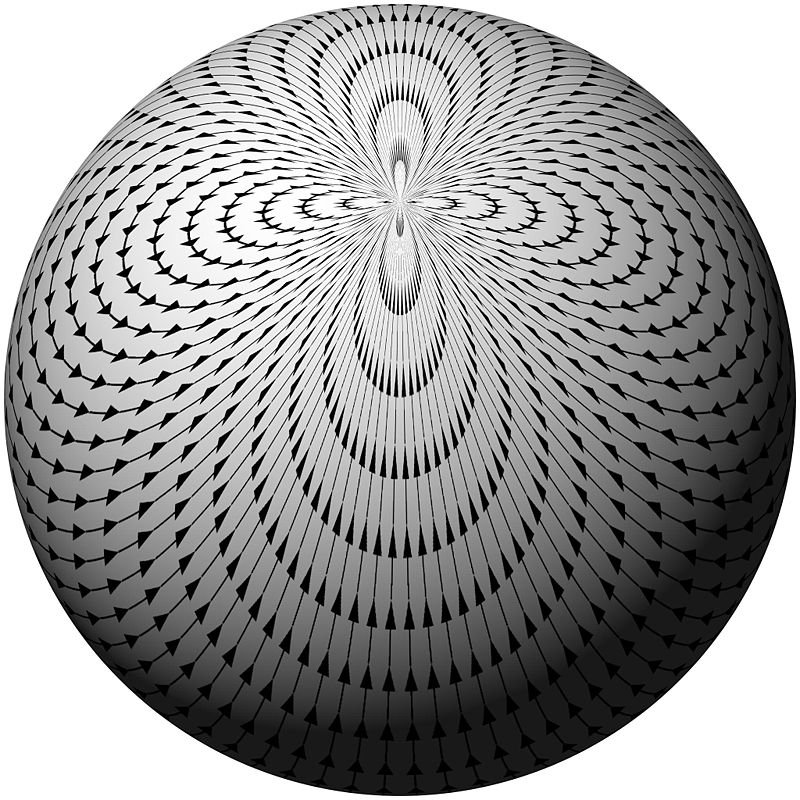
\includegraphics[width=0.4\textwidth]{Images/hairyball}
  \caption{An isolated singular point guaranteed by the Poincar\'e-Hopf
    theorem\footnotemark}
\end{figure}   
    \footnotetext{Image Courtesy of Wikipedia: RokerHRO - Own work, CC BY-SA 3.0,
    \url{https://commons.wikimedia.org/w/index.php?curid=8257798}}
\begin{theorem}[The Hairy Ball Theorem] You can't comb a hairy ball without
  a bald spot. Or, in more precise terms, let $f$ be a continuous function
  that assigns a vector in $\mathbb{R}^3$ to each point on $S^2$, such that
  $f(p)$ is tangent to $S^2$ at $p$. Then, there is at least one $p$ for
  such that $f(p)=0$.
\end{theorem}
\begin{proof}
  Assume, in order to find a contradiction, that $f(p)\neq 0$ for all $p$ on
  the 2-sphere. Then, there exists a vector field $v$ on $S^2$ such that $v$
  has no singular points. However, given the above theorem, this is
  a contradiction, as we know that there must exist two distinct isolated
  singular points on this vector field, thusly there can be no such vector
  field on the sphere or on any manifold topologically homeomorphic to the
  sphere.
\end{proof}
asdsadd
